\subsubsection{How does the autoencoder work?}
Autoencoders are neural networks designed to learn efficient representations of data by compressing input through an encoder, capturing essential features in a compact bottleneck layer, and reconstructing the original data using a decoder. Rather than simply memorizing inputs, autoencoders aim to capture the underlying structure or essence of the data, similar to how students rephrase and recall learned material during exams. In the context of a diabetes dataset, an autoencoder can be a powerful tool for feature extraction. By training the autoencoder on the dataset, we can compress high-dimensional input data into a lower-dimensional latent representation that retains meaningful patterns related to diabetes. These extracted features can then be used for tasks like classification, clustering, or anomaly detection, potentially improving performance and interpretability by focusing on the most informative aspects of the data.\\

\noindent An autoencoder is not a god match for a classification task as in our case. But, it can be used as a tool for feature extraction, together with a classification algorithm. And this is what we have done in our case. We used an autoencoder with one encode layer and one decode layer and than used Gradient Boosting Classifer for the prediction. This kind of solution achieved an accuracy of 74$\%$ and a recall of 79$\%$. This is not an outstanding performance, but also not a bad estimation.
We have provided a diagram of our encoder in figure \ref{fig:autoencoder}. This shows the input items, the encoding and decoding step determining the structure.\\


\begin{figure}[h]
    \centering
    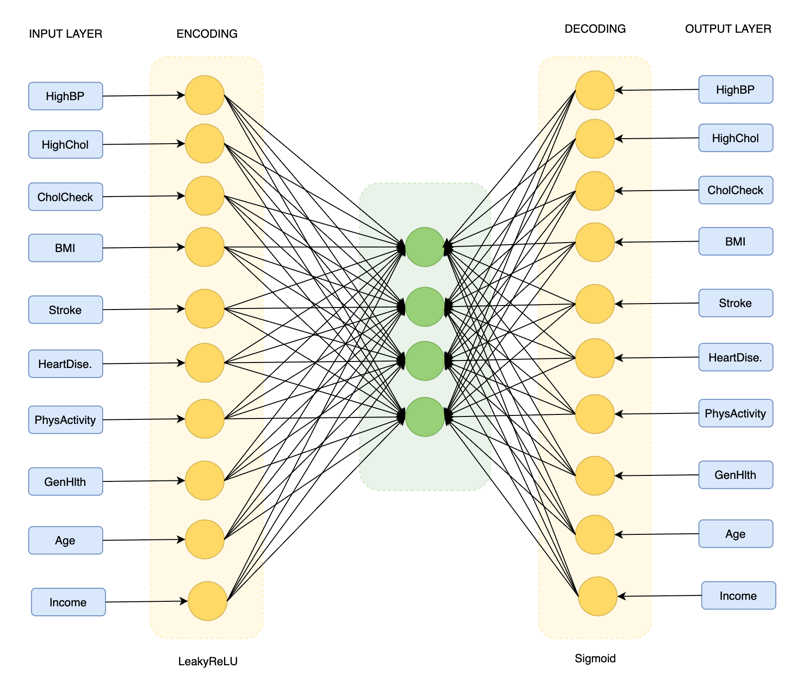
\includegraphics[width=0.7\textwidth]{images/autoencoder.png}
    \caption{Autoencoder Architecture}
    \label{fig:autoencoder}
\end{figure}

\subsubsection{Finding the best match for the parameters}
In order to try the best algorithms and the best parameters we had tried many combinations on the dataset.
First we tested the four classifiers as listed on table \ref{tab:alg}. Than after deciding that Gradient Boosting Classifer performed best, we have tested 32 possible combinations, out of wich there is a 10 $\%$ difference, quite a considerable accuracy difference.
All the tested algorithms and their recall is listed on the 4 below tables: \ref{tab:op1},\ref{tab:op2},\ref{tab:op3},\ref{tab:op4}.

\begin{table}[H]
    \centering
    \begin{tabular}{|l|c|}
        \hline
        \textbf{Function} & \textbf{Accuracy} \\
        \hline
        Logistic Regression & 68\% \\
        Random Forest Classifier & 66\% \\
        Gradient Boosting Classifier & 74\% \\
        SVC (RBF Kernel) & 69\% \\
        \hline
    \end{tabular}
    \caption{Accuracy of Various Classification Models}
    \label{tab:alg}
\end{table}


\begin{table}[H]
    \centering
    \begin{tabular}{|c|c|c|c|c|c|c|}
        \hline
        \rowcolor{lightgreen}
        \textbf{Model} & \textbf{Activation} & \textbf{Optimizer} & \textbf{Loss} & \textbf{Learning Rate} & \textbf{Accuracy} & \textbf{Recall} \\
        \hline
        Model 1 & ReLU & Adam & MSE & 0.1 & 0.7212 & 0.7212 \\
        \hline
        Model 2 & ReLU & Adam & MSE & 0.3 & 0.7231 & 0.7231 \\
        \hline
        Model 3 & ReLU & Adam & Binary CE & 0.1 & 0.6974 & 0.6974 \\
        \hline
        Model 4 & ReLU & Adam & Binary CE & 0.3 & 0.6947 & 0.6947 \\
        \hline
        Model 5 & ReLU & SGD & MSE & 0.1 & 0.6915 & 0.6915 \\
        \hline
        Model 6 & ReLU & SGD & MSE & 0.3 & 0.7017 & 0.7017 \\
        \hline
        Model 7 & ReLU & SGD & Binary CE & 0.1 & 0.6880 & 0.6880 \\
        \hline
        Model 8 & ReLU & SGD & Binary CE & 0.3 & 0.6868 & 0.6868 \\
        \hline
    \end{tabular}
    \caption{Parameter testing for autoencoder}
    \label{tab:op1}
\end{table}
\begin{table}[H]
    \centering
    \begin{tabular}{|c|c|c|c|c|c|c|}
        \hline
        \rowcolor{lightgreen}
        \textbf{Model} & \textbf{Activation} & \textbf{Optimizer} & \textbf{Loss} & \textbf{Learning Rate} & \textbf{Accuracy} & \textbf{Recall} \\
        \hline
        Model 9 & Sigmoid & Adam & MSE & 0.1 & 0.5 & 0.5 \\
        \hline
        Model 10 & Sigmoid & Adam & MSE & 0.3 & 0.5 & 0.5 \\
        \hline
        Model 11 & Sigmoid & Adam & Binary CE & 0.1 & 0.7021 & 0.7021 \\
        \hline
        Model 12 & Sigmoid & Adam & Binary CE & 0.3 & 0.7210 & 0.7210 \\
        \hline
        Model 13 & Sigmoid & SGD & MSE & 0.1 & 0.7200 & 0.7200 \\
        \hline
        Model 14 & Sigmoid & SGD & MSE & 0.3 & 0.7215 & 0.7215 \\
        \hline
        Model 15 & Sigmoid & SGD & Binary CE & 0.1 & -- & -- \\
        \hline
        Model 16 & Sigmoid & SGD & Binary CE & 0.3 & -- & -- \\
        \hline
    \end{tabular}
    \caption{Parameter testing for autoencoder}
    \label{tab:op2}
\end{table}
\begin{table}[H]
    \centering
    \begin{tabular}{|c|c|c|c|c|c|c|}
        \hline
        \rowcolor{lightgreen}
        \textbf{Model} & \textbf{Activation} & \textbf{Optimizer} & \textbf{Loss} & \textbf{Learning Rate} & \textbf{Accuracy} & \textbf{Recall} \\
        \hline
        Model 17 & Leaky ReLU & Adam & MSE & 0.1 & 0.7415 & 0.7415 \\
        \hline
        Model 18 & Leaky ReLU & Adam & MSE & 0.3 & 0.7417 & 0.7417 \\
        \hline
        Model 19 & Leaky ReLU & Adam & Binary CE & 0.1 & 0.7157 & 0.7157 \\
        \hline
        Model 20 & Leaky ReLU & Adam & Binary CE & 0.3 & 0.7153 & 0.7153 \\
        \hline
        Model 21 & Leaky ReLU & SGD & MSE & 0.1 & 0.7024 & 0.7024 \\
        \hline
        Model 22 & Leaky ReLU & SGD & MSE & 0.3 & 0.7019 & 0.7019 \\
        \hline
        Model 23 & Leaky ReLU & SGD & Binary CE & 0.1 & 0.7364 & 0.7364 \\
        \hline
        Model 24 & Leaky ReLU & SGD & Binary CE & 0.3 & 0.7320 & 0.7320 \\
        \hline
    \end{tabular}
    \caption{Parameter testing for autoencoder}
    \label{tab:op3}
\end{table}
\begin{table}[H]
    \centering
    \begin{tabular}{|c|c|c|c|c|c|c|}
        \hline
        \rowcolor{lightgreen}
        \textbf{Model} & \textbf{Activation} & \textbf{Optimizer} & \textbf{Loss} & \textbf{Learning Rate} & \textbf{Accuracy} & \textbf{Recall} \\
        \hline
        Model 17 & Leaky ReLU & Adam & MSE & 0.1 & 0.7415 & 0.7415 \\
        \hline
        Model 18 & Leaky ReLU & Adam & MSE & 0.3 & 0.7417 & 0.7417 \\
        \hline
        Model 19 & Leaky ReLU & Adam & Binary CE & 0.1 & 0.7157 & 0.7157 \\
        \hline
        Model 20 & Leaky ReLU & Adam & Binary CE & 0.3 & 0.7153 & 0.7153 \\
        \hline
        Model 21 & Leaky ReLU & SGD & MSE & 0.1 & 0.7024 & 0.7024 \\
        \hline
        Model 22 & Leaky ReLU & SGD & MSE & 0.3 & 0.7019 & 0.7019 \\
        \hline
        Model 23 & Leaky ReLU & SGD & Binary CE & 0.1 & 0.7364 & 0.7364 \\
        \hline
        Model 24 & Leaky ReLU & SGD & Binary CE & 0.3 & 0.7320 & 0.7320 \\
        \hline
    \end{tabular}
    \caption{Parameter testing for autoencoder}
    \label{tab:op4}
\end{table}





\subsubsection{Implementation}
In order to implement the autoencoder, we will use the \codebox{keras} library. The autoencoder will only function as a feature extractor, for the classification task we will need the {GradientBoostingClassifier} from \codebox{sklearn} library.\\

\noindent The dataset is used the same as for the other algorithms, from the training and testing files.

\vspace{0.5cm}
\lstinputlisting[language=python]{../code/autoencoder/separate_code_for_report/preparation.py}
\vspace{0.5cm}

\noindent Next, the Autoencoder class contains all the logic for the feature extraction task. First the input layer is constructed from keras.layer library. Than encoder is built from the Dense method, also from the keras library, together with the LeakyReLU decoder. The autoencoder is parametrized with the input layer, and two optimization functions are given. Lastly the model is trained with the training set and a batch size of 32. After all the preparations, the model should be trained with the testin set part. The last step will be running the model encoding for the testing set.

\vspace{0.5cm}
\lstinputlisting[language=python]{../code/autoencoder/separate_code_for_report/autoencoder_class.py}
\vspace{0.5cm}

\noindent The remaining step will be running the algorithm.
We will first instantiate an encoder from the class we just built, using leaky relu for the first activation function and sigmoid for the second.
As optimizer functions adam and mse are used.
Encoding dim is set to four, for the four attributes to be mapped to, and 50 epochs are used for training.
The output of the encoder is passed to Gradient Boosting Classifer, for the prediction task.
To finish off, we print the confusion matrix, since in our case, as it was also mentioned before, the recall plays a more important role than the accuracy, so this step is unevitable.\\

\vspace{0.5cm}
\lstinputlisting[language=python]{../code/autoencoder/separate_code_for_report/usage.py}
\vspace{0.5cm}

\noindent The result after running the code above are given on the table \ref{tab:autoencoder_classification_report}.

\begin{figure}[h!]
    \centering
    \begin{minipage}[b]{0.4\textwidth}
        \centering
        \begin{tabular}{lcccc}
            \hline
            \textbf{Class} & \textbf{Precision} & \textbf{Recall} & \textbf{F1-Score} & \textbf{Support} \\
            \hline
            0.0 & 0.77 & 0.68 & 0.72 & 10604 \\
            1.0 & 0.71 & 0.79 & 0.75 & 10604 \\
            \hline
            \textbf{Accuracy} & \multicolumn{3}{c}{0.74} & 21208 \\
            \textbf{Macro Avg} & 0.74 & 0.74 & 0.74 & 21208 \\
            \textbf{Weighted Avg} & 0.74 & 0.74 & 0.74 & 21208 \\
            \hline
        \end{tabular}
        \caption{Classification Report for Autoencoder}
        \label{tab:autoencoder_classification_report}

        \vspace{1.5cm}
    \end{minipage}
    \hfill
    \begin{minipage}[b]{0.4\textwidth}
        \centering
        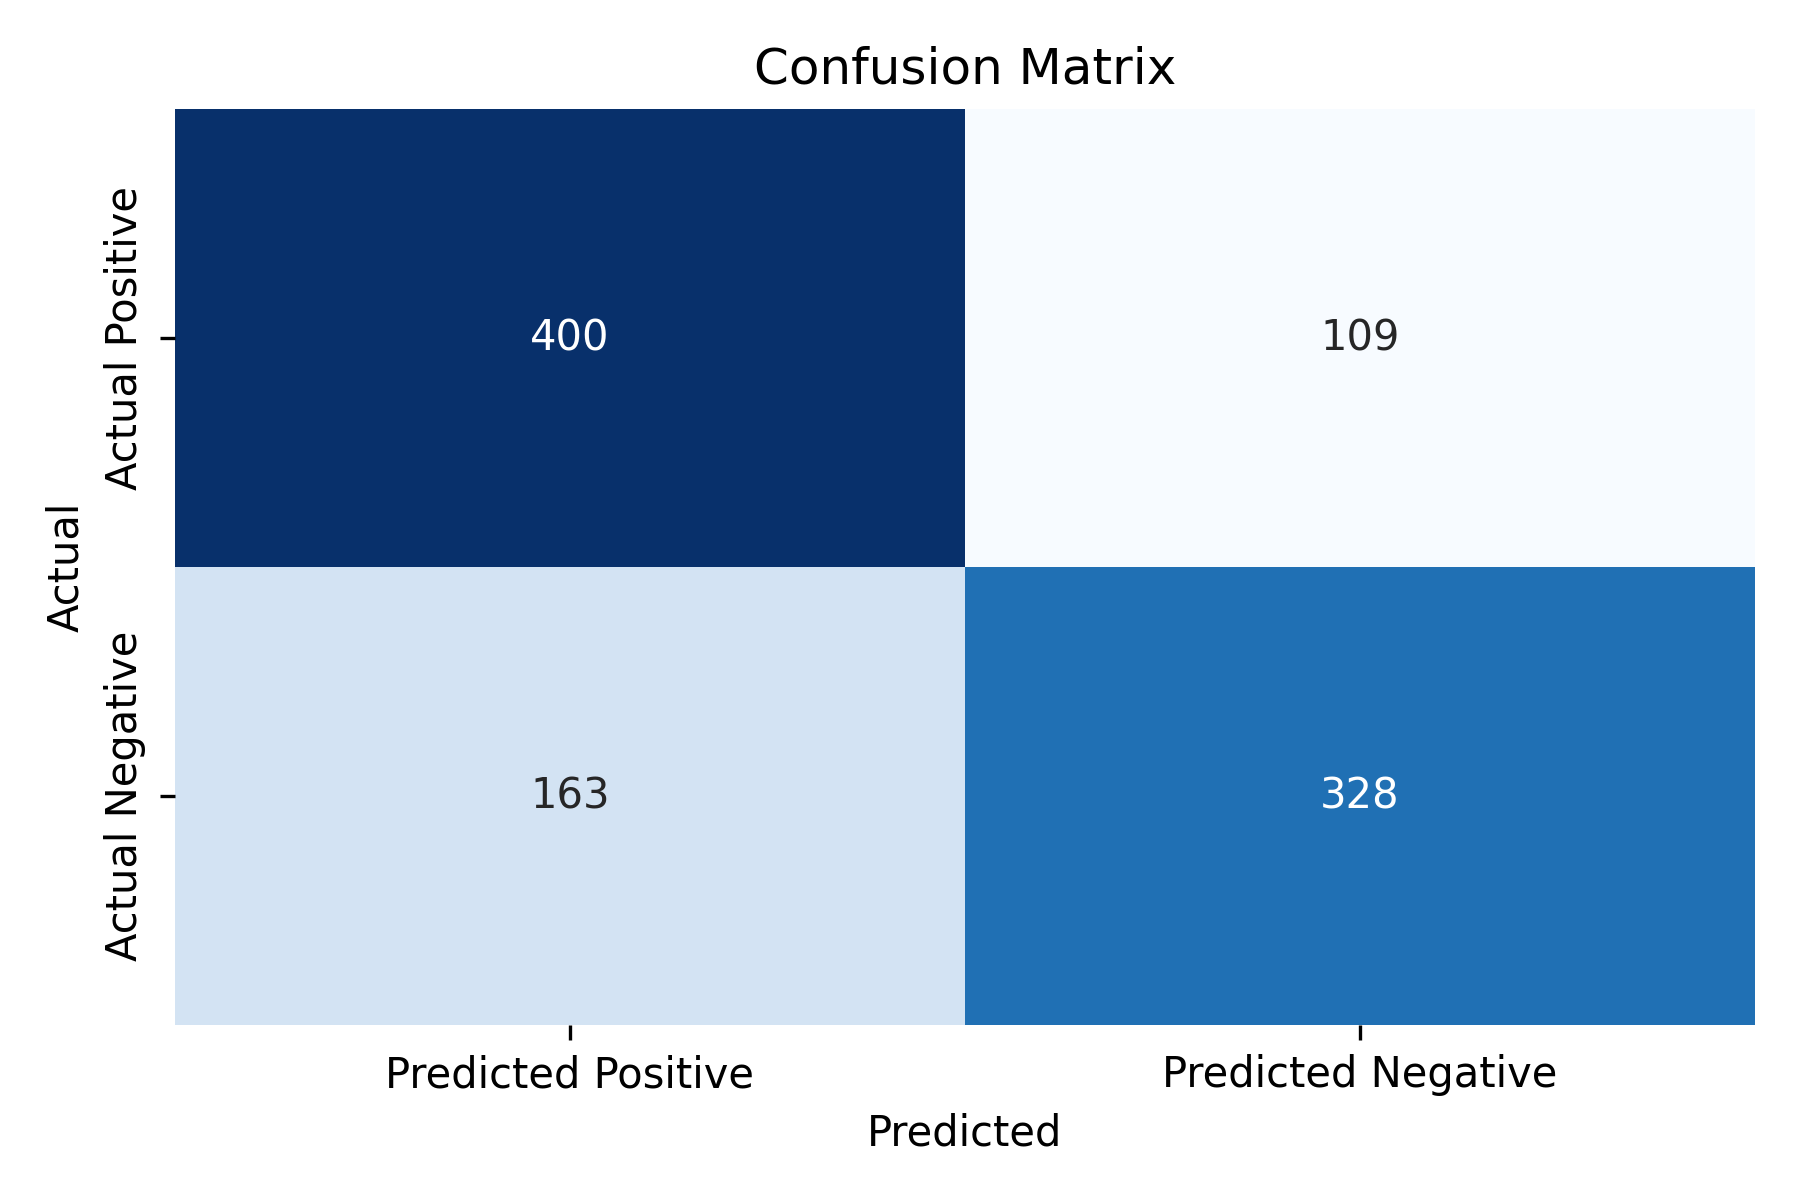
\includegraphics[width=\textwidth]{images/autoencoder_confusion_matrix.png}
        \caption{Autoencoder Confusion Matrix}
        \label{fig:autoencoder_cfm}
    \end{minipage}
\end{figure}